%-*- mode: LaTeX; -*-

\chapter{Discussion}
\label{sec:discussion}
This chapter discusses the results presented in chapter \ref{sec:results}. The chapter is divided into two parts, one part discusses the results of seed growth and the other part discusses the results from characterization of the B-doped samples. 

\section{Seed growth}
As shown in section \ref{sec:results:seeds}, the carbon face grown seeds did not have complete coverage of cubic SiC on the terrace, yet the silicon face grown seeds could reproducibly be grown with complete cubic coverage. As seen in figure \ref{fig:supersaturation}, 2D growth is promoted by high supersaturation. A possible explanation of the results is that the supersaturation for the C-face growth was too low. The examined temperatures, as shown in table \ref{tab:seeds}  range from 1825 to 1925 $^\circ$C, which is a large portion of the parameter space in which the 3C-SiC polytype is stable. Changing the temperature much more during growth is unlikely to result in better 3C-coverage, since this will likely be outside the region where 3C-SiC can be formed in a stable manner. Because of this, the supersaturation will not be able to be changed much more by altering the temperature. 

From table \ref{tab:seeds} it can be seen that the percentage of the terrace covered by 3C-SiC does not show any trend with regards to temperature. The growth time has been adjusted to get similar sample thickness for all samples. In this way it was possible to vary only the supersaturation between samples. This indicates that for the used growth setup it is not possible to change the supersaturation enough to get complete 3C-SiC coverage of the terrace. However, the pressure conditions for growth have not been explored in this work, and it may be possible to alter the ambient pressure to get more cubic coverage. 

A possible explanation of the difference in 3C-SiC coverage on silicon and carbon face substrates is the spiral growth character. On Si-face the spirals take the form of proper spirals, with steps expanding from the spiral arms. The C-face spiral takes the form of straight lines extending radially from the center, as seen in figure \ref{fig:carbon_seed1}. The 3C-SiC polytype nucleates on top of the heteroepitaxially grown spirals and grows over the spiral steps. The spiral shape can then be expected to influence how the 3C-SiC is grown. The silicon face spiral may be advantageous for cubic growth, while the carbon face spiral may not be. Another possible explanation is that there may be some difference between how the Si- and C-surfaces look for off-axis cut samples. There may be a difference in the number and density of the steps, which in turn will influence the terrace growth. To get a proper understanding of this, electron microscopy would have to be done on the substrate surface and the terrace after initial nucleation. In this way a proper understanding of the growth mechanisms governing C- and Si-face growth would be possible. This is beyond the scope of this work, but could be included in future work. 

The silicon and carbon faces have different surface energies which will influence how material grows on it. Stein et al. have shown that SiC growth on 4H-SiC and 6H-SiC substrates will result in different polytypes grown depending on the face rather than the substrate polytype. This they attributed to the different surface energies of the different faces \cite{Stein1992}. This may also be a factor in the problem of growing 3C-SiC on the carbon face. From the micrographs of the carbon face seeds it can be seen that cubic growth always occurs at the edge of the facet, i.e. near the graphite spacer. This is consistent with the hypothesis that the surface energy gives rise to the results since the edge is expected to have a different surface energy compared to somewhere towards the center of the sample. 

%\begin{itemize}
%\item Possible explanation is that the supersaturation is too low (see graph). Supersaturation varies with temperature, we should see a trend when varying temperature. We do not. 
%\item Cannot vary temperature much more, since 3C is only stable in small temperature window. 
%\item Spiral shape is different, maybe this shape is not good for 2D-growth. 
%\item C and Si has different surface energies, which will influence growth. Maybe the C conditions are not compatible with the 3C-growth. 
%\item The surface energy alternative explains why we always see 3C at the edge, never in the center.  
%\end{itemize}

\section{B-doped samples}
From figure \ref{fig:B_doped_micrographs1} it can clearly be seen that B-doping deteriorates the crystal quality. All doped samples have a larger number of defects compared to the nominally undoped sample. For samples D1 and D4 the number of defects increase with increasing source doping. This is to be expected since the boron atoms have a different radius compared to both the silicon and carbon atoms they replace. This size difference will induce strain in the sample and in turn induce defects. From the same figure we can see that sample D6, which was grown with the source material with the highest doping concentration, has a smoother surface compared to the two other doped samples characterized in this thesis. This does not follow the trend. In figure \ref{fig:BGe20_micrograph} (b) can be seen that sample D9, grown from the same source material as D6, shows similarly good surface quality. In contrast sample D8, again grown from the same source material, has a much poorer surface. From the absorption measurements on these samples it can be inferred that these materials do not in fact have very good quality. As described in chapter \ref{sec:results}, samples D8 and D9 do not show any B-CB absorption peak, and D6 does not show the band edge absorption. One possible explanation of this is that the source material does not in fact have the high doping concentration it is thought to have. This hypothesis is contradicted by the result of absorption measurement on D6. If the samples would be only lightly doped, then the band edge absorption would still be visible. Another possible explanation is that even though the surface shows a low density of defects, the sample may be of poor crystal quality. This would explain why sample D6 does not show any band edge absorption. Further characterization of the crystal quality of these samples would give more insight to why the surfaces seem smooth but the absorption measurements yield poor results. 

Figure \ref{fig:B_doped_micrographs2} shows the difference in surface morphology of doped samples D1 and D8, which have been grown using the direct and indirect growth methods, respectively. The fact that they both show similar numbers of surface defects could indicate that both samples have been doped with comparable concentrations of boron. As shown earlier a higher concentration of boron will induce more defects on the surface. Figure \ref{fig:abs} (b) gives a further indication that this hypothesis is valid. This figure indicates that the two samples give similar absorption spectra. Most importantly both spectra show the B-CB peak at around 700 nm. From this it can be suggested that the indirect doping method introduced in this work is able to introduce impurities in a grown sample. The density of introduced impurities is from the results thought to be similar, but methods better suited to give impurity concentrations should be used to validate this finding. 

The doped samples D1-D5 and D8 all show band edge absorption and the B-CB absorption peak, but none of the samples shows the VB-B peak, which should be present at around 1700 nm. A possible explanation for this would be that the B-level is near or below the Fermi level, so that the occupancy of the level is too high to show much absorption. The Fermi level can be computed if the doping concentrations are known. It can be assumed that the nitrogen doping concentration is the same in doped samples as in unintentionally doped samples, i.e. the donor concentration is $N_D \approx 10^{16}$ cm$^{-3}$. Assuming that the B-doped samples are of p-type, i.e. $p>>n$, the neutrality condition is
\begin{equation}
\label{eq:neutrality1}
p = N_A^- - N_D^+.
\end{equation}
Since the nitrogen energy level is shallow, it can be assumed that at room temperature all donor atoms are ionized. This gives that $N_D^+ =N_D$. Under the Boltzmann approximation the hole density is
\begin{equation}
\label{eq:p}
p \approx N_Ve^{-E_F/kT},
\end{equation}
were $N_V$ is the valence band density of states, and is given by
\begin{equation}
\label{eq:nv}
N_V = 2\left(\frac{kTm_{d,h}}{2\pi \hbar^2}\right)^{3/2},
\end{equation}
where $m_{d,h}$ is the density of states hole mass. The number of ionized acceptor atoms is governed by the temperature and the distance between the Fermi level and the acceptor level, 
\begin{equation}
\label{eq:ionized}
N_A^- = \frac{N_A}{1+2e^{\frac{E_A-E_F}{kT}}}.
\end{equation}
From equations \ref{eq:p}-\ref{eq:ionized} the neutrality condition \ref{eq:neutrality1} can be rewritten as
\begin{equation}
\label{eq:neutrality2}
f(E_F) \equiv N_Ve^{-E_F/kT}+2N_Ve^{(E_A-2E_F)/kT}+2N_De^{(E_A-E_F)/kT} - N_A + N_D = 0,
\end{equation}
where the LHS is denoted $f(E_F)$. By using the values $E_A = 0.735$ meV, $m_{d,h} = 0.6m_0$ and $T = 300$ K, equation \ref{eq:neutrality2} gives the plots in figures \ref{fig:N_A} and \ref{fig:fermi}. In \ref{fig:N_A}, the graphs show the function $f(E_F)$ for different values of $N_A$, ranging from $10^{17}$ (light blue) to $10^{18}$ (dark blue) cm$^{-3}$. In figure \ref{fig:fermi} the Fermi level has been computed for concentrations ranging from $10^{16}$ to $10^{21}$ cm$^{-3}$. It can be seen that for concentration around 3$\times10^{17}$ cm$^{-3}$, the Fermi level is at 0.74 eV, which corresponds to the acceptor level. It is likely that the doping concentration in the sample is in the same order of magnitude, or smaller, as in the source material from which it was grown. From this it can be concluded that for doped samples grown with source impurity concentration of $10^{18}$ the Fermi level likely is near or above the acceptor level at room temperature. If the doping concentration of grown samples is significantly smaller than of the source material, then it is probable that also the samples grown from $10^{19}$ and $10^{20}$ cm$^{-3}$ sources have the Fermi level above the acceptor level. This may be the reason why the VB-B peak is not visible in the absorption spectra. 

\begin{figure}[h]
\centering
\begin{minipage}{.5\textwidth}
  \centering
  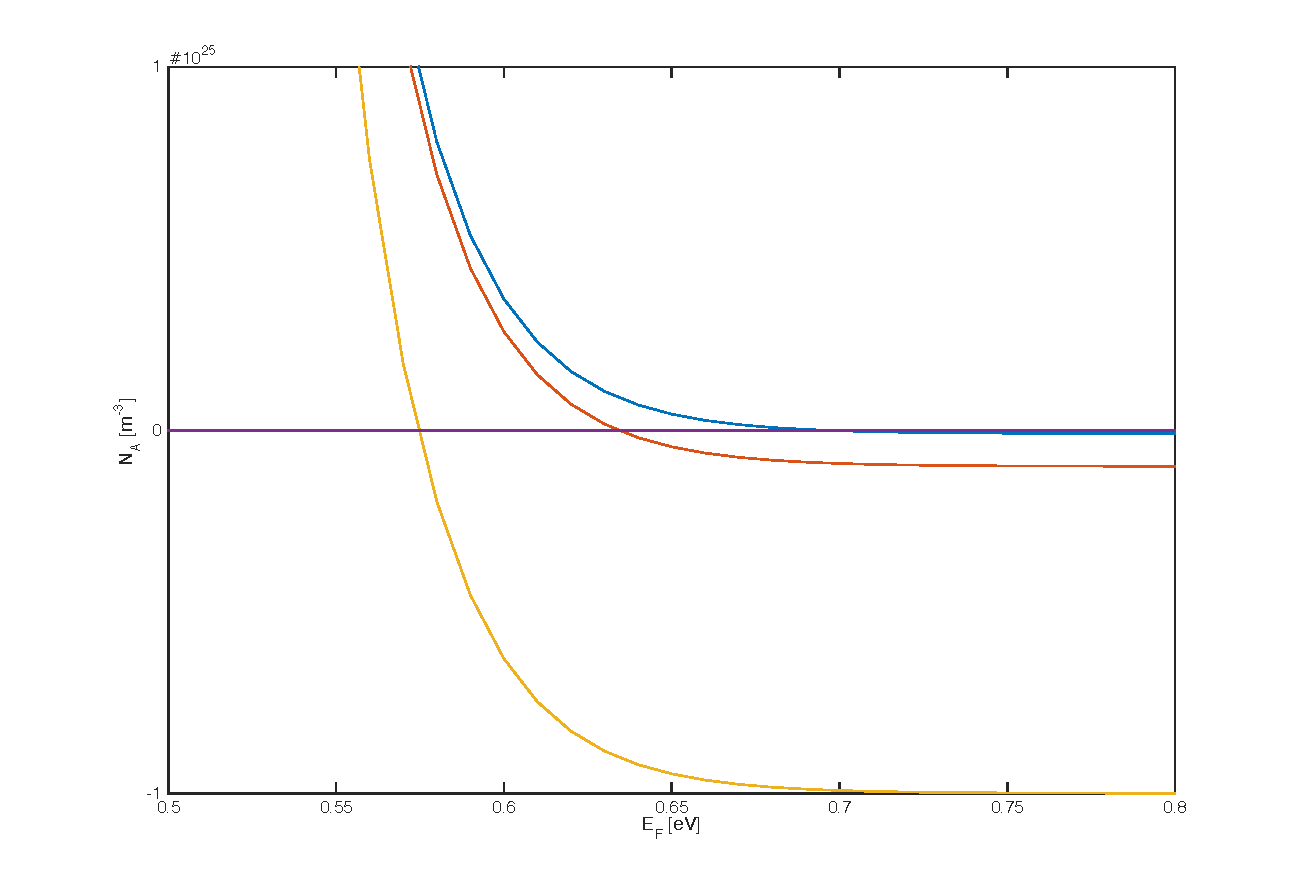
\includegraphics[scale=0.3]{N_A.pdf}
  \captionof{figure}{Computed values of LHS in equation \ref{eq:neutrality2}, plotted against the Fermi level. The three graphs show acceptor concentrations of $10^{17}$, $10^{18}$ and $10^{19}$ cm$^{-3}$. }
  \label{fig:N_A}
\end{minipage}%
\begin{minipage}{.5\textwidth}
  \centering
  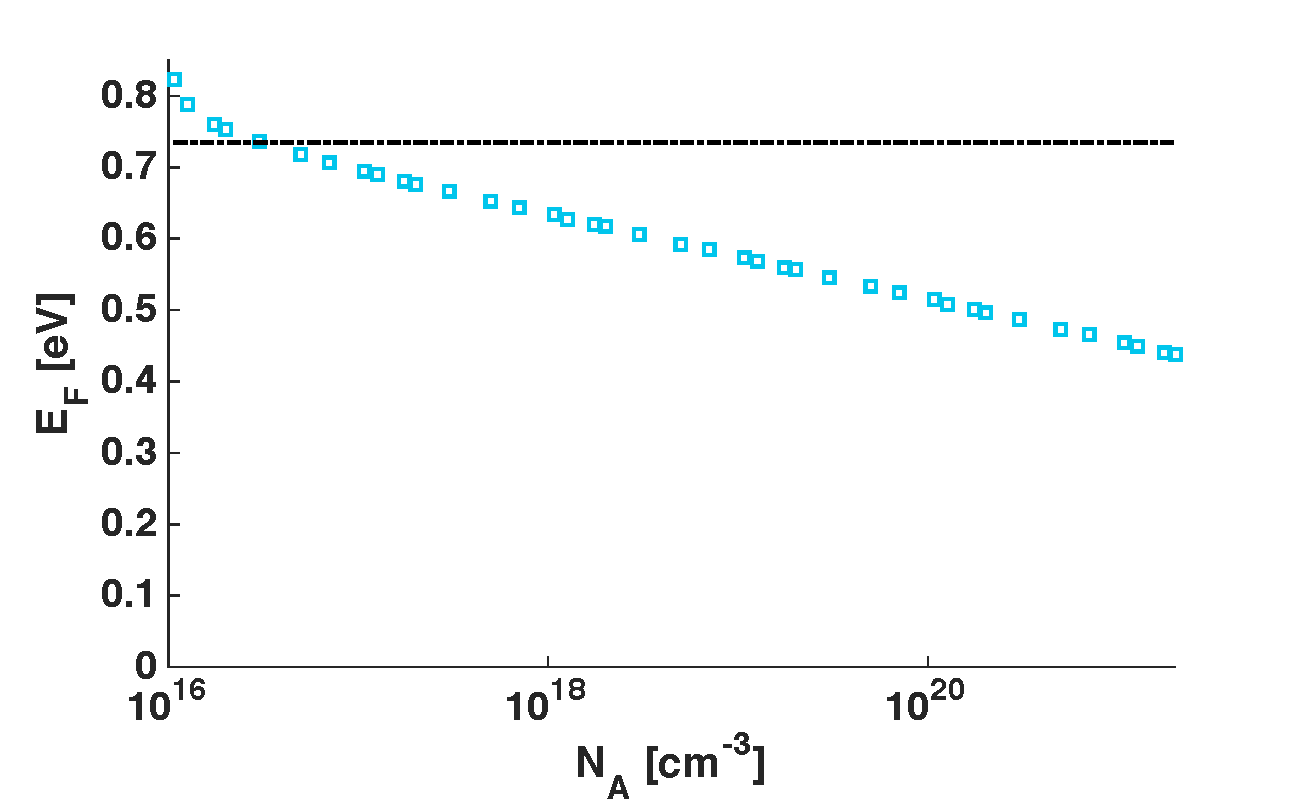
\includegraphics[scale=0.4]{Fermi.pdf}
  \captionof{figure}{Calculations of the Fermi level for different acceptor atom concentrations}
  \label{fig:fermi}
\end{minipage}
\end{figure}

Most of the B-doped samples showed no luminescence at all. One possible explanation for this is that the acceptor level is of non-radiative character. It is to be expected that boron, which is a deep level impurity, is of non-radiative character and recombines in a way which does not emit a photon, such as by the Shockley-Reed-Hall process \cite{Hall1952,Shockley1952}. There have, however, been reports of luminescence from B-doping levels in 3C-SiC, for example by Kubawara  et al. \cite{Company1976}. This means that the fact that the B-level may be to some extent non-radiative does not entirely explain why most of the doped samples measured show no luminescence. 

Another explanation of the PL-spectra from the doped samples is that the boron doped samples are not of sufficient crystal quality. As shown in figure \ref{fig:B_doped_micrographs1} the doped samples contain many defects. It may be that the many defects form non-radiative levels in the band gap and which compete with the boron level. This would explain why the results do not agree to those reported in literature. 

One sample (D9) did show luminescence at around 6000 Å which corresponds to an aluminium impurity level. As aluminium is a shallow acceptor, it will be able to capture carriers more easily compared to the deep levels created by boron. It is likely that more carriers are captured in the Al-level, which decreases the number of exciton recombinations from the B-level. This may be another explanation of why no boron related lines can be seen. There is luminescence from the hexagonal inclusions in this sample (inclusions are shown in figure \ref{fig:BGe20_micrograph} (c)). The luminescence is thought to originate from the B-CB transition. It is likely that both polytypes in the same sample have similar impurity concentrations for both B and Al. This is not consistent with the hypothesis that B-Al competition is responsible for the lack of B-lines in the 3C-SiC spectra. 













































